\begin{pastexam}[label={px:ntu-110-bime-ds-01}]{臺大生機所 110 學年度 第 1 題}
（問答；10 分）

(10\%) Write down the sequence of the 7 keys in the array that results after performing 3 successive
delete-the-max operations on the following maximum-oriented \textbf{binary heap} of size 10:\\
\hspace*{1em}97 82 89 34 66 78 85 15 28 51
\end{pastexam}

\begin{pastsoln}
答案：82 66 78 34 15 28 51。

陣列從索引 1 開始，節點 $i$ 的子節點是 $2i$、$2i+1$。 刪除最大值的做法照資結書第~8.1~節
（虛擬碼~8.2）：拿走根，把最後一個鍵搬到根，堆積大小減一，再從根往下調整（和比較大的子節點比，
比它小就交換）。 先畫出原來的堆積：
\begin{center}
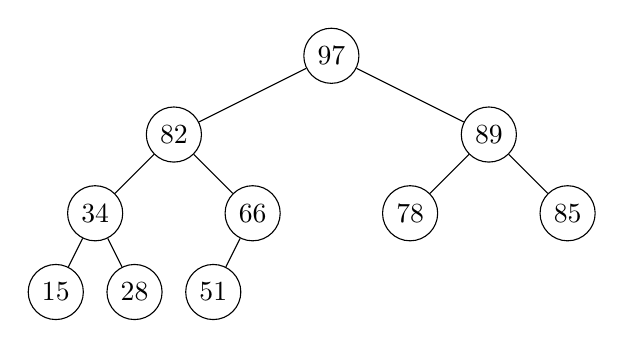
\begin{tikzpicture}[v/.style={circle,draw,inner sep=1pt,minimum size=7mm},
  level distance=10mm, level 1/.style={sibling distance=40mm},
  level 2/.style={sibling distance=20mm}, level 3/.style={sibling distance=10mm}]
\node[v] {97}
  child {node[v] {82}
    child {node[v] {34} child {node[v] {15}} child {node[v] {28}}}
    child {node[v] {66} child {node[v] {51}} child[missing] {}}}
  child {node[v] {89}
    child {node[v] {78}}
    child {node[v] {85}}};
\end{tikzpicture}
\end{center}

\textbf{第 1 次}：拿走 97，最後一個 51 搬到根，大小 9。
\begin{itemize}[nosep]
\item 根 51 的子節點 82、89，較大的是 89，$51 < 89$，交換，51 到索引 3。
\item 索引 3 的子節點（索引 6、7）是 78、85，較大的 85，$51 < 85$，交換，51 到索引 7，沒有子節點，停。
\end{itemize}
陣列：89 82 85 34 66 78 51 15 28。

\textbf{第 2 次}：拿走 89，最後一個 28 搬到根，大小 8。
\begin{itemize}[nosep]
\item 根 28 的子節點 82、85，和 85 交換，28 到索引 3。
\item 索引 3 的子節點 78、51，和 78 交換，28 到索引 6，沒有子節點（$2\cdot 6 > 8$），停。
\end{itemize}
陣列：85 82 78 34 66 28 51 15。

\textbf{第 3 次}：拿走 85，最後一個 15 搬到根，大小 7。
\begin{itemize}[nosep]
\item 根 15 的子節點 82、78，和 82 交換，15 到索引 2。
\item 索引 2 的子節點（索引 4、5）是 34、66，和 66 交換，15 到索引 5，沒有子節點（$2\cdot 5 > 7$），停。
\end{itemize}
陣列：82 66 78 34 15 28 51。

整理成表（粗體是這次往下調整走過的位置）：
\begin{center}
\begin{tabular}{lcccccccccc}
\toprule
 & 1 & 2 & 3 & 4 & 5 & 6 & 7 & 8 & 9 & 10 \\
\midrule
原來 & 97 & 82 & 89 & 34 & 66 & 78 & 85 & 15 & 28 & 51 \\
刪 97 後 & \textbf{89} & 82 & \textbf{85} & 34 & 66 & 78 & \textbf{51} & 15 & 28 & \\
刪 89 後 & \textbf{85} & 82 & \textbf{78} & 34 & 66 & \textbf{28} & 51 & 15 & & \\
刪 85 後 & \textbf{82} & \textbf{66} & 78 & 34 & \textbf{15} & 28 & 51 & & & \\
\bottomrule
\end{tabular}
\end{center}
最後檢查：82 的子節點 66、78；66 的子節點 34、15；78 的子節點 28、51，都滿足最大堆積的性質。
\end{pastsoln}
